\documentclass[uplatex,a4j]{jsreport}
\usepackage{thesis}

\begin{document}
\chapter{HTML5字句解析器}
\section{HTML5字句解析仕様書}
HTML5字句解析仕様はWHATWG communityのwebサイトから得られる.~\cite{html5specification}
HTML5の字句解析仕様には80個の状態がある.
\begin{figure}[h]
    \centering
    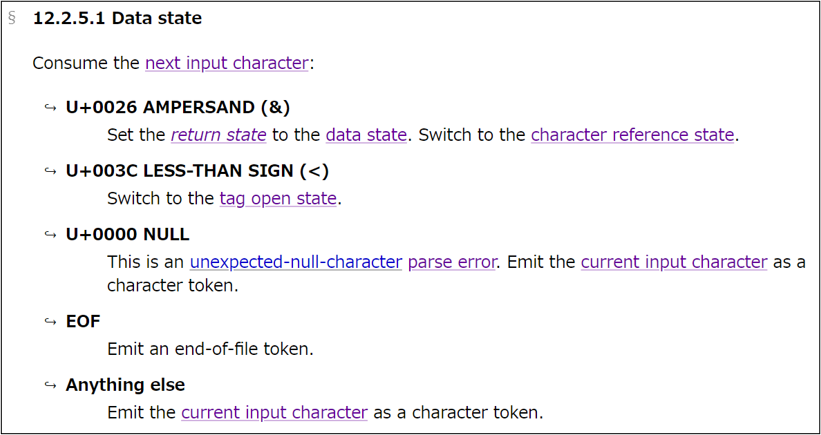
\includegraphics[keepaspectratio, scale=1.0]
         {figure/html5.png}
    \caption{HTML5字句解析仕様書}
    \label{html5}
\end{figure}
   aaa図\ref{html5}

%% BNF
\section{BNF}
$cList$ : CommandList\\
c : Command\\
b : Bool\\
cval : CommandValue\\
ival : InplementVariable\\
\begin{eqnarray*}
    {\rm cList }&\bnfdef& c :: cList \bnfor Nil\\
\end{eqnarray*}
\begin{eqnarray*}
    {\rm c }&::=& \mbox{if $\langle$Bool$\rangle$ then $\langle$cList$\rangle_1$ else $\langle$cList$\rangle_2$}\\
      &|& \mbox{ Ignore() //} \\
      &|& \mbox{ Switch($\langle$CommandValue$\rangle$)} \\
      &|& \mbox{ Reconsume($\langle$CommandValue$\rangle$)} \\
      &|& \mbox{ Set(<ImplementVariable>, $\langle$CommandValue$\rangle$)} \\
      &|& \mbox{ AppendTo($\langle$CommandValue$\rangle$, <ImplementVariable>)} \\
      &|& \mbox{ Emit($\langle$CommandValue$\rangle$)} \\
      &|& \mbox{ Create($\langle$CommandValue$\rangle$)} \\
      &|& \mbox{ Consume($\langle$CommandValue$\rangle$)} \\
      &|& \mbox{ Error($\langle$CommandValue$\rangle$)} \\
      &|& \mbox{ FlushCodePoint()} \\
      &|& \mbox{ StartAttribute()} \\
      &|& \mbox{ TreatAsAnythingElse()} \\
      &|& \mbox{ AddTo($\langle$CommandValue$\rangle$, $\langle$ImplementVariable$\rangle$) 
                //$\langle$ImplementVariable$\rangle = \langle$ImplementVariable$\rangle + \langle$CommandValue$\rangle$ } \\
      &|& \mbox{ MultiplyBy(<ImplementVariable>, $\langle$CommandValue$\rangle$)} \\
\end{eqnarray*}
\begin{eqnarray*}
    {\rm <Bool> }&::=& And(<Bool>, <Bool>)\\
      &|& Or(<Bool>, <Bool>) \\
      &|& Not(<Bool>) \\
      &|& CharacterReferenceConsumedAsAttributeVal() \\
      &|& CurrentEndTagIsAppropriate() \\
      &|& IsEqual(<CommandValue>, <CommandValue>) \\
\end{eqnarray*}
\begin{eqnarray*}
    {\rm b }&::=& \mbox{ And}(b_1, b_2)\\
      &|& \mbox{ Or}(b_1, b_2) \\
      &|& \mbox{ Not}(b) \\
      &|& \mbox{ CharacterReferenceConsumedAsAttributeVal}() \mbox{ // CharacterReferenceCodeが属性の値として消費されているか} \\
      &|& \mbox{ CurrentEndTagIsAppropriate}() \mbox{ //EndTagTokenが適切であるか } \\
      &|& \mbox{ IsEqual}(cval_1, cval_2) \\
\end{eqnarray*}

\begin{eqnarray*}
    {\rm <CommandValue> }&::=& StateName(<String>)\\
      &|& ReturnState \\
      &|& TemporaryBuffer \\
      &|& CharacterReferenceCode \\
      &|& NewStartTagToken \\
      &|& NewEndTagToken \\
      &|& NewDOCTYPEToken \\
      &|& NewCommentToken \\
      &|& CurrentTagToken \\
      &|& CurrentDOCTYPEToken \\
      &|& CurrentAttribute \\
      &|& CommentToken \\
      &|& EndOfFileToken \\
      &|& CharacterToken(<Char>) \\
      &|& LowerCase(<CommandValue>) \\
      &|& NumericVersion(<CommandValue>) \\
      &|& CurrentInputCharacter \\
      &|& NextInputCharacter \\
      &|& Variable(<String>) \\
      &|& CChar(<Char>) \\
      &|& CString(<String>) \\
      &|& CInt(<Int>) \\
      &|& CBool(<Boolean>) \\
\end{eqnarray*}
\begin{eqnarray*}
    {\rm <ImplementVariable> }&::=& IReturnState\\
      &|& ITemporaryBuffer \\
      &|& ICharacterReferenceCode \\
      &|& ICurrentTagToken \\
      &|& ICurrentDOCTYPEToken \\
      &|& ICurrentAttribute \\
      &|& ICommentToken \\
      &|& IVariable(<String>) \\
      &|& INameOf(<ImplementVariable>) \\
      &|& IValueOf(<ImplementVariable>) \\
      &|& IFlagOf(<ImplementVariable>) \\
      &|& SystemIdentifierOf(<ImplementVariable>) \\
      &|& PublicIdentifierOf(<ImplementVariable>) \\
\end{eqnarray*}
\end{document}